% Options for packages loaded elsewhere
\PassOptionsToPackage{unicode}{hyperref}
\PassOptionsToPackage{hyphens}{url}
\PassOptionsToPackage{dvipsnames,svgnames,x11names}{xcolor}
%
\documentclass[
  letterpaper,
  DIV=11,
  numbers=noendperiod]{scrartcl}

\usepackage{amsmath,amssymb}
\usepackage{iftex}
\ifPDFTeX
  \usepackage[T1]{fontenc}
  \usepackage[utf8]{inputenc}
  \usepackage{textcomp} % provide euro and other symbols
\else % if luatex or xetex
  \usepackage{unicode-math}
  \defaultfontfeatures{Scale=MatchLowercase}
  \defaultfontfeatures[\rmfamily]{Ligatures=TeX,Scale=1}
\fi
\usepackage{lmodern}
\ifPDFTeX\else  
    % xetex/luatex font selection
\fi
% Use upquote if available, for straight quotes in verbatim environments
\IfFileExists{upquote.sty}{\usepackage{upquote}}{}
\IfFileExists{microtype.sty}{% use microtype if available
  \usepackage[]{microtype}
  \UseMicrotypeSet[protrusion]{basicmath} % disable protrusion for tt fonts
}{}
\makeatletter
\@ifundefined{KOMAClassName}{% if non-KOMA class
  \IfFileExists{parskip.sty}{%
    \usepackage{parskip}
  }{% else
    \setlength{\parindent}{0pt}
    \setlength{\parskip}{6pt plus 2pt minus 1pt}}
}{% if KOMA class
  \KOMAoptions{parskip=half}}
\makeatother
\usepackage{xcolor}
\usepackage[top=30mm,left=30mm]{geometry}
\setlength{\emergencystretch}{3em} % prevent overfull lines
\setcounter{secnumdepth}{-\maxdimen} % remove section numbering
% Make \paragraph and \subparagraph free-standing
\makeatletter
\ifx\paragraph\undefined\else
  \let\oldparagraph\paragraph
  \renewcommand{\paragraph}{
    \@ifstar
      \xxxParagraphStar
      \xxxParagraphNoStar
  }
  \newcommand{\xxxParagraphStar}[1]{\oldparagraph*{#1}\mbox{}}
  \newcommand{\xxxParagraphNoStar}[1]{\oldparagraph{#1}\mbox{}}
\fi
\ifx\subparagraph\undefined\else
  \let\oldsubparagraph\subparagraph
  \renewcommand{\subparagraph}{
    \@ifstar
      \xxxSubParagraphStar
      \xxxSubParagraphNoStar
  }
  \newcommand{\xxxSubParagraphStar}[1]{\oldsubparagraph*{#1}\mbox{}}
  \newcommand{\xxxSubParagraphNoStar}[1]{\oldsubparagraph{#1}\mbox{}}
\fi
\makeatother

\usepackage{color}
\usepackage{fancyvrb}
\newcommand{\VerbBar}{|}
\newcommand{\VERB}{\Verb[commandchars=\\\{\}]}
\DefineVerbatimEnvironment{Highlighting}{Verbatim}{commandchars=\\\{\}}
% Add ',fontsize=\small' for more characters per line
\usepackage{framed}
\definecolor{shadecolor}{RGB}{241,243,245}
\newenvironment{Shaded}{\begin{snugshade}}{\end{snugshade}}
\newcommand{\AlertTok}[1]{\textcolor[rgb]{0.68,0.00,0.00}{#1}}
\newcommand{\AnnotationTok}[1]{\textcolor[rgb]{0.37,0.37,0.37}{#1}}
\newcommand{\AttributeTok}[1]{\textcolor[rgb]{0.40,0.45,0.13}{#1}}
\newcommand{\BaseNTok}[1]{\textcolor[rgb]{0.68,0.00,0.00}{#1}}
\newcommand{\BuiltInTok}[1]{\textcolor[rgb]{0.00,0.23,0.31}{#1}}
\newcommand{\CharTok}[1]{\textcolor[rgb]{0.13,0.47,0.30}{#1}}
\newcommand{\CommentTok}[1]{\textcolor[rgb]{0.37,0.37,0.37}{#1}}
\newcommand{\CommentVarTok}[1]{\textcolor[rgb]{0.37,0.37,0.37}{\textit{#1}}}
\newcommand{\ConstantTok}[1]{\textcolor[rgb]{0.56,0.35,0.01}{#1}}
\newcommand{\ControlFlowTok}[1]{\textcolor[rgb]{0.00,0.23,0.31}{\textbf{#1}}}
\newcommand{\DataTypeTok}[1]{\textcolor[rgb]{0.68,0.00,0.00}{#1}}
\newcommand{\DecValTok}[1]{\textcolor[rgb]{0.68,0.00,0.00}{#1}}
\newcommand{\DocumentationTok}[1]{\textcolor[rgb]{0.37,0.37,0.37}{\textit{#1}}}
\newcommand{\ErrorTok}[1]{\textcolor[rgb]{0.68,0.00,0.00}{#1}}
\newcommand{\ExtensionTok}[1]{\textcolor[rgb]{0.00,0.23,0.31}{#1}}
\newcommand{\FloatTok}[1]{\textcolor[rgb]{0.68,0.00,0.00}{#1}}
\newcommand{\FunctionTok}[1]{\textcolor[rgb]{0.28,0.35,0.67}{#1}}
\newcommand{\ImportTok}[1]{\textcolor[rgb]{0.00,0.46,0.62}{#1}}
\newcommand{\InformationTok}[1]{\textcolor[rgb]{0.37,0.37,0.37}{#1}}
\newcommand{\KeywordTok}[1]{\textcolor[rgb]{0.00,0.23,0.31}{\textbf{#1}}}
\newcommand{\NormalTok}[1]{\textcolor[rgb]{0.00,0.23,0.31}{#1}}
\newcommand{\OperatorTok}[1]{\textcolor[rgb]{0.37,0.37,0.37}{#1}}
\newcommand{\OtherTok}[1]{\textcolor[rgb]{0.00,0.23,0.31}{#1}}
\newcommand{\PreprocessorTok}[1]{\textcolor[rgb]{0.68,0.00,0.00}{#1}}
\newcommand{\RegionMarkerTok}[1]{\textcolor[rgb]{0.00,0.23,0.31}{#1}}
\newcommand{\SpecialCharTok}[1]{\textcolor[rgb]{0.37,0.37,0.37}{#1}}
\newcommand{\SpecialStringTok}[1]{\textcolor[rgb]{0.13,0.47,0.30}{#1}}
\newcommand{\StringTok}[1]{\textcolor[rgb]{0.13,0.47,0.30}{#1}}
\newcommand{\VariableTok}[1]{\textcolor[rgb]{0.07,0.07,0.07}{#1}}
\newcommand{\VerbatimStringTok}[1]{\textcolor[rgb]{0.13,0.47,0.30}{#1}}
\newcommand{\WarningTok}[1]{\textcolor[rgb]{0.37,0.37,0.37}{\textit{#1}}}

\providecommand{\tightlist}{%
  \setlength{\itemsep}{0pt}\setlength{\parskip}{0pt}}\usepackage{longtable,booktabs,array}
\usepackage{calc} % for calculating minipage widths
% Correct order of tables after \paragraph or \subparagraph
\usepackage{etoolbox}
\makeatletter
\patchcmd\longtable{\par}{\if@noskipsec\mbox{}\fi\par}{}{}
\makeatother
% Allow footnotes in longtable head/foot
\IfFileExists{footnotehyper.sty}{\usepackage{footnotehyper}}{\usepackage{footnote}}
\makesavenoteenv{longtable}
\usepackage{graphicx}
\makeatletter
\def\maxwidth{\ifdim\Gin@nat@width>\linewidth\linewidth\else\Gin@nat@width\fi}
\def\maxheight{\ifdim\Gin@nat@height>\textheight\textheight\else\Gin@nat@height\fi}
\makeatother
% Scale images if necessary, so that they will not overflow the page
% margins by default, and it is still possible to overwrite the defaults
% using explicit options in \includegraphics[width, height, ...]{}
\setkeys{Gin}{width=\maxwidth,height=\maxheight,keepaspectratio}
% Set default figure placement to htbp
\makeatletter
\def\fps@figure{htbp}
\makeatother

\KOMAoption{captions}{tableheading}
\makeatletter
\@ifpackageloaded{caption}{}{\usepackage{caption}}
\AtBeginDocument{%
\ifdefined\contentsname
  \renewcommand*\contentsname{Table of contents}
\else
  \newcommand\contentsname{Table of contents}
\fi
\ifdefined\listfigurename
  \renewcommand*\listfigurename{List of Figures}
\else
  \newcommand\listfigurename{List of Figures}
\fi
\ifdefined\listtablename
  \renewcommand*\listtablename{List of Tables}
\else
  \newcommand\listtablename{List of Tables}
\fi
\ifdefined\figurename
  \renewcommand*\figurename{Figure}
\else
  \newcommand\figurename{Figure}
\fi
\ifdefined\tablename
  \renewcommand*\tablename{Table}
\else
  \newcommand\tablename{Table}
\fi
}
\@ifpackageloaded{float}{}{\usepackage{float}}
\floatstyle{ruled}
\@ifundefined{c@chapter}{\newfloat{codelisting}{h}{lop}}{\newfloat{codelisting}{h}{lop}[chapter]}
\floatname{codelisting}{Listing}
\newcommand*\listoflistings{\listof{codelisting}{List of Listings}}
\makeatother
\makeatletter
\makeatother
\makeatletter
\@ifpackageloaded{caption}{}{\usepackage{caption}}
\@ifpackageloaded{subcaption}{}{\usepackage{subcaption}}
\makeatother

\ifLuaTeX
  \usepackage{selnolig}  % disable illegal ligatures
\fi
\usepackage{bookmark}

\IfFileExists{xurl.sty}{\usepackage{xurl}}{} % add URL line breaks if available
\urlstyle{same} % disable monospaced font for URLs
\hypersetup{
  pdftitle={2. Data Discovery},
  pdfauthor={Cob Staines},
  colorlinks=true,
  linkcolor={blue},
  filecolor={Maroon},
  citecolor={Blue},
  urlcolor={Blue},
  pdfcreator={LaTeX via pandoc}}


\title{2. Data Discovery}
\author{Cob Staines}
\date{2024-11-08}

\begin{document}
\maketitle

\renewcommand*\contentsname{Table of contents}
{
\hypersetup{linkcolor=}
\setcounter{tocdepth}{3}
\tableofcontents
}

\emph{This tutorial is available as a
\href{https://github.com/RIBBiTR-BII/ribbitr-data-access/tree/main/tutorial_series}{.qmd
on Github}.}

\section{Motivation}\label{motivation}

\begin{itemize}
\tightlist
\item
  Explore what data are currently available on the database
\item
  Identify structure of data of interest to inform access
\end{itemize}

\section{R}

Let's set up our environment to get ready to explore the database.

\subsection{Load packages}\label{load-packages}

\begin{Shaded}
\begin{Highlighting}[]
\CommentTok{\# minimal packages for RIBBiTR DB data discovery}
\NormalTok{librarian}\SpecialCharTok{::}\FunctionTok{shelf}\NormalTok{(tidyverse, dbplyr, RPostgres, DBI, RIBBiTR}\SpecialCharTok{{-}}\NormalTok{BII}\SpecialCharTok{/}\NormalTok{ribbitrrr)}
\end{Highlighting}
\end{Shaded}

\subsection{Establish database
connection}\label{establish-database-connection}

\begin{Shaded}
\begin{Highlighting}[]
\CommentTok{\# establish database connection}
\NormalTok{dbcon }\OtherTok{=} \FunctionTok{hopToDB}\NormalTok{(}\StringTok{"ribbitr"}\NormalTok{)}
\end{Highlighting}
\end{Shaded}

\begin{verbatim}
Connecting to database... Success!
\end{verbatim}

\subsection{Load database metadata}\label{load-database-metadata}

\subsubsection{Data structure: Schemas, tables, columns and
rows}\label{data-structure-schemas-tables-columns-and-rows}

The RIBBiTR database is organized into ``schemas'' (think of these as
folders), which can contain any number of tables. Each table consists of
columns (``variables'') and rows (``entries'').

\subsubsection{Metadata: Data about
data}\label{metadata-data-about-data}

We keep track of information regarding what tables, and columns exist in
the database, and what information they are designed to describe, using
table and column metadata. To begin our process of data discovery, let's
learn what tables are present in the data by loading the table metadata.

\subsubsection{Table Metadata}\label{table-metadata}

\begin{Shaded}
\begin{Highlighting}[]
\CommentTok{\# load table "all\_tables" from schema "public"}
\NormalTok{mdt }\OtherTok{=} \FunctionTok{tbl}\NormalTok{(dbcon, }\FunctionTok{Id}\NormalTok{(}\StringTok{"public"}\NormalTok{, }\StringTok{"all\_tables"}\NormalTok{)) }\SpecialCharTok{\%\textgreater{}\%}
  \FunctionTok{collect}\NormalTok{()}
\end{Highlighting}
\end{Shaded}

\paragraph{Some basic database
commands}\label{some-basic-database-commands}

Before we take a look at the metadata you just pulled, let's understand
the command we just ran.

\begin{itemize}
\tightlist
\item
  \texttt{dplyr::tbl()} - This function is used to create a ``lazy''
  table from a data source. To specify the source, we provide the
  database connection \texttt{dbcon}, as well as a pointer or
  ``address'' for the table of interest using the \texttt{Id()}
  function. A ``lazy'' table means that the data only pulled when
  explicitly asked for. See \texttt{collect()} below.
\item
  \texttt{dbplyr::Id()} - This function is a pointer to pass
  hierarchical table identifiers (you can think of this as an address
  for a given table). In this case we use it to generate an pointer for
  the table ``all\_tables'' in schema ``public''.
\item
  \texttt{dplyr::collect()} - the \texttt{tbl()} function generates a
  ``lazy'' table, which is basically a shopping list for the data you
  want to pull. In order to actually pull the data from the server to
  your local machine (ie. ``do the shopping'') we need to pipe in the
  \texttt{collect()} function.
\end{itemize}

\textbf{Also try:} Run the code above without \texttt{collect()}, to see
what a lazy table looks like.

Now let's take a look at the table metadata to explore what schemas and
tables exist.

\begin{Shaded}
\begin{Highlighting}[]
\FunctionTok{view}\NormalTok{(mdt)}
\end{Highlighting}
\end{Shaded}

\subsubsection{Column metadata}\label{column-metadata}

Suppose our interest is in the \texttt{survey\_data} schema. Let's take
a closer look at the tables here by collecting metadata on table columns
in this schema.

\begin{Shaded}
\begin{Highlighting}[]
\CommentTok{\# load table "all\_columns" from schema "public"}
\NormalTok{mdc }\OtherTok{=} \FunctionTok{tbl}\NormalTok{(dbcon, }\FunctionTok{Id}\NormalTok{(}\StringTok{"public"}\NormalTok{, }\StringTok{"all\_columns"}\NormalTok{)) }\SpecialCharTok{\%\textgreater{}\%}
  \FunctionTok{filter}\NormalTok{(table\_schema }\SpecialCharTok{==} \StringTok{"survey\_data"}\NormalTok{) }\SpecialCharTok{\%\textgreater{}\%}
  \FunctionTok{collect}\NormalTok{()}
\end{Highlighting}
\end{Shaded}

Notice we used the \texttt{dplyr::filter()} command on the lazy table
\emph{before} running \texttt{collect()}. This effectively revised the
shopping list before going to the store, rather than bringing home the
entire store and then filtering for what you want in your kitchen. Much
less (computationally) expensive!

Let's check out the column metadata, and see what you can learn.

\begin{Shaded}
\begin{Highlighting}[]
\FunctionTok{view}\NormalTok{(mdc)}

\CommentTok{\# list the columns in our column{-}metadata table}
\FunctionTok{colnames}\NormalTok{(mdc)}
\end{Highlighting}
\end{Shaded}

\begin{verbatim}
 [1] "table_schema"             "table_name"              
 [3] "column_name"              "definition"              
 [5] "units"                    "accuracy"                
 [7] "scale"                    "format"                  
 [9] "natural_key"              "reviewed"                
[11] "data_type"                "character_maximum_length"
[13] "numeric_precision"        "datetime_precision"      
[15] "is_nullable"              "column_default"          
[17] "ordinal_position"         "pg_description"          
[19] "key_type"                
\end{verbatim}

Curious about what a certain metadata column means? There's metadata for
that (metametadata?)!

\begin{Shaded}
\begin{Highlighting}[]
\CommentTok{\# vew metadata on metadata columns}
\FunctionTok{view}\NormalTok{(mdc }\SpecialCharTok{\%\textgreater{}\%} \FunctionTok{filter}\NormalTok{(table\_name }\SpecialCharTok{==} \StringTok{"metadata\_columns"}\NormalTok{))}
\end{Highlighting}
\end{Shaded}

A few columns to point out:

\begin{itemize}
\tightlist
\item
  definition
\item
  units
\item
  data\_type
\item
  natural key
\end{itemize}

(more on keys later)

\subsection{Our first(?) data table}\label{our-first-data-table}

Ok, let's try to apply some of what we have learned by pulling directly
from a data table. We can begin by taking a look at the visual encounter
surveys (VES).

\begin{Shaded}
\begin{Highlighting}[]
\CommentTok{\# create lazy table for ves (visual encounter survey) table}
\NormalTok{db\_ves }\OtherTok{=} \FunctionTok{tbl}\NormalTok{(dbcon, }\FunctionTok{Id}\NormalTok{(}\StringTok{"survey\_data"}\NormalTok{, }\StringTok{"ves"}\NormalTok{))}
\end{Highlighting}
\end{Shaded}

Do these functions look familiar? Turns out, we were pulling data all
along! Of course, this is a lazy table (ie. shopping list) so it doesn't
look like data yet. Let's see what we can learn from it before going to
the store to collect the data.

What columns the table contains:

\begin{Shaded}
\begin{Highlighting}[]
\CommentTok{\# return columns of lazy table}
\FunctionTok{colnames}\NormalTok{(db\_ves)}
\end{Highlighting}
\end{Shaded}

\begin{verbatim}
 [1] "species_ves"         "count_ves"           "detection_location" 
 [4] "microhab"            "life_stage"          "sex"                
 [7] "comments_ves"        "microhab_moredetail" "observer_ves"       
[10] "visual_animal_state" "ves_id"              "survey_id"          
\end{verbatim}

How many total rows a table contains:

\begin{Shaded}
\begin{Highlighting}[]
\CommentTok{\# count rows}
\NormalTok{db\_ves }\SpecialCharTok{\%\textgreater{}\%}
  \FunctionTok{summarise}\NormalTok{(}\AttributeTok{row\_count =} \FunctionTok{n}\NormalTok{()) }\SpecialCharTok{\%\textgreater{}\%}
  \FunctionTok{pull}\NormalTok{(row\_count)}
\end{Highlighting}
\end{Shaded}

\begin{verbatim}
integer64
[1] 28390
\end{verbatim}

\emph{The pull() function executes a query to return a single column or
variable, synonymous with the collect() function which returns a
collection of variables as a table.}

How many rows after filtering for unknown species:

\begin{Shaded}
\begin{Highlighting}[]
\CommentTok{\# count rows with known species}
\NormalTok{db\_ves }\SpecialCharTok{\%\textgreater{}\%}
  \FunctionTok{filter}\NormalTok{(}\SpecialCharTok{!}\FunctionTok{is.na}\NormalTok{(species\_ves),}
\NormalTok{         species\_ves }\SpecialCharTok{!=} \StringTok{"unknown\_species"}\NormalTok{) }\SpecialCharTok{\%\textgreater{}\%}
  \FunctionTok{summarise}\NormalTok{(}\AttributeTok{row\_count =} \FunctionTok{n}\NormalTok{()) }\SpecialCharTok{\%\textgreater{}\%}
  \FunctionTok{pull}\NormalTok{(row\_count)}
\end{Highlighting}
\end{Shaded}

\begin{verbatim}
integer64
[1] 28232
\end{verbatim}

How many rows corresponding to a each life stage:

\begin{Shaded}
\begin{Highlighting}[]
\CommentTok{\# count rows by life stage}
\NormalTok{db\_ves }\SpecialCharTok{\%\textgreater{}\%}
  \FunctionTok{select}\NormalTok{(life\_stage) }\SpecialCharTok{\%\textgreater{}\%}
  \FunctionTok{group\_by}\NormalTok{(life\_stage) }\SpecialCharTok{\%\textgreater{}\%}
  \FunctionTok{summarise}\NormalTok{(}\AttributeTok{row\_count =} \FunctionTok{n}\NormalTok{()) }\SpecialCharTok{\%\textgreater{}\%}
  \FunctionTok{arrange}\NormalTok{(}\FunctionTok{desc}\NormalTok{(row\_count)) }\SpecialCharTok{\%\textgreater{}\%}
  \FunctionTok{collect}\NormalTok{()}
\end{Highlighting}
\end{Shaded}

\begin{verbatim}
# A tibble: 8 x 2
  life_stage row_count
  <chr>        <int64>
1 tadpole        10276
2 adult           9551
3 subadult        7162
4 <NA>             764
5 eggmass          625
6 egg                9
7 juvenile           2
8 metamorph          1
\end{verbatim}

\subsection{Also try}\label{also-try}

\section{Python}

Let's set up our environment to get ready to explore the database.

\subsection{Load packages}\label{load-packages-1}

\begin{Shaded}
\begin{Highlighting}[]
\CommentTok{\# minimal packages for Python DB data discovery}
\ImportTok{import}\NormalTok{ ibis}
\ImportTok{from}\NormalTok{ ibis }\ImportTok{import}\NormalTok{ \_}
\ImportTok{import}\NormalTok{ pandas }\ImportTok{as}\NormalTok{ pd}
\ImportTok{import}\NormalTok{ dbconfig}
\end{Highlighting}
\end{Shaded}

\subsection{Establish database
connection}\label{establish-database-connection-1}

\begin{Shaded}
\begin{Highlighting}[]
\CommentTok{\# Establish database connection}
\NormalTok{dbcon }\OperatorTok{=}\NormalTok{ ibis.postgres.}\ExtensionTok{connect}\NormalTok{(}\OperatorTok{**}\NormalTok{dbconfig.ribbitr)}
\end{Highlighting}
\end{Shaded}

\subsection{Load database metadata}\label{load-database-metadata-1}

\subsubsection{Data structure: Schemas, tables, columns and
rows}\label{data-structure-schemas-tables-columns-and-rows-1}

The RIBBiTR database is organized into ``schemas'' (think of these as
folders), which can contain any number of tables. Each table consists of
columns (``variables'') and rows (``entries'').

\subsubsection{Metadata: Data about
data}\label{metadata-data-about-data-1}

We keep track of information regarding what tables, and columns exist in
the database, and what information they are designed to describe, using
table and column metadata. To begin our process of data discovery, let's
learn what tables are present in the data by loading the table metadata.

\subsubsection{Table Metadata}\label{table-metadata-1}

\begin{Shaded}
\begin{Highlighting}[]
\CommentTok{\# load table "all\_tables" from schema "public"}
\NormalTok{mdt }\OperatorTok{=}\NormalTok{ dbcon.table(database }\OperatorTok{=} \StringTok{"public"}\NormalTok{, name }\OperatorTok{=} \StringTok{"all\_tables"}\NormalTok{).to\_pandas()}
\end{Highlighting}
\end{Shaded}

\paragraph{Some basic database
commands}\label{some-basic-database-commands-1}

Before we take a look at the metadata you just pulled, let's understand
the command we just ran.

\begin{itemize}
\tightlist
\item
  \texttt{ibis.table()} - This function is used to create a ``lazy''
  table from a data source. To specify the source, we modify the
  database connection \texttt{dbcon}. We specify the schema for the
  table as \texttt{public} (note ibis calls this ``database''), as well
  as the table name \texttt{all\_tables}. A ``lazy'' table means that
  the data only pulled when explicitly asked for. See \texttt{execute()}
  below.
\item
  \texttt{ibis.to\_pandas()} - the \texttt{table()} function generates a
  ``lazy'' table, which is basically a shopping list for the data you
  want to pull. In order to actually pull the data from the server to
  your local machine (ie. ``do the shopping'') we need to collect the
  lazy table by chaining the \texttt{to\_pandas()} function.
\end{itemize}

\textbf{Also try:} Run the code above without \texttt{to\_pandas()}, to
see what an uncollected lazy table looks like.

Now let's take a look at the table metadata to explore what schemas and
tables exist.

\begin{Shaded}
\begin{Highlighting}[]
\BuiltInTok{print}\NormalTok{(mdt)}
\end{Highlighting}
\end{Shaded}

\begin{verbatim}
   table_schema          table_name  column_count table_description
0      bay_area      amphib_dissect            41              None
1      bay_area     amphib_parasite            11              None
2      bay_area  water_quality_info            27              None
3      bay_area                site            25              None
4      bay_area        wetland_info            25              None
..          ...                 ...           ...               ...
58     kira_pep              survey            17              None
59     kira_pep                 ves             9              None
60     kira_pep             capture            24              None
61     kira_pep     metadata_tables             4              None
62     kira_pep    metadata_columns            19              None

[63 rows x 4 columns]
\end{verbatim}

\subsubsection{Column metadata}\label{column-metadata-1}

Suppose our interest is in the \texttt{survey\_data} schema. Let's take
a closer look at the tables here by collecting metadata on table columns
in this schema.

\begin{Shaded}
\begin{Highlighting}[]
\CommentTok{\# load table "all\_columns" from schema "public"}
\NormalTok{mdc }\OperatorTok{=}\NormalTok{ (}
\NormalTok{  dbcon.table(database}\OperatorTok{=}\StringTok{"public"}\NormalTok{, name}\OperatorTok{=}\StringTok{"all\_columns"}\NormalTok{)}
\NormalTok{  .}\BuiltInTok{filter}\NormalTok{(\_.table\_schema }\OperatorTok{==} \StringTok{\textquotesingle{}survey\_data\textquotesingle{}}\NormalTok{)}
\NormalTok{  .to\_pandas()}
\NormalTok{)}
\end{Highlighting}
\end{Shaded}

Notice we used the \texttt{ibis.filter()} command on the lazy table
\emph{before} calling \texttt{to\_pandas()}. This effectively revised
the shopping list before going to the store, rather than bringing home
the entire store and then filtering for what you want in your kitchen.
Much less (computationally) expensive!

Let's check out the column metadata, and see what you can learn.

\begin{Shaded}
\begin{Highlighting}[]
\CommentTok{\# view dataframe}
\BuiltInTok{print}\NormalTok{(mdc)}
\end{Highlighting}
\end{Shaded}

\begin{verbatim}
    table_schema        table_name  ... pg_description key_type
0    survey_data              site  ...           None     None
1    survey_data              site  ...           None     None
2    survey_data              site  ...           None     None
3    survey_data           capture  ...           None     None
4    survey_data  metadata_columns  ...           None       PK
..           ...               ...  ...            ...      ...
335  survey_data               ves  ...           None     None
336  survey_data               ves  ...           None     None
337  survey_data               ves  ...           None     None
338  survey_data               ves  ...           None     None
339  survey_data               ves  ...           None       FK

[340 rows x 19 columns]
\end{verbatim}

\begin{Shaded}
\begin{Highlighting}[]
\CommentTok{\# list the columns in our column{-}metadata table}
\NormalTok{mdc.columns}
\end{Highlighting}
\end{Shaded}

\begin{verbatim}
Index(['table_schema', 'table_name', 'column_name', 'definition', 'units',
       'accuracy', 'scale', 'format', 'natural_key', 'reviewed', 'data_type',
       'character_maximum_length', 'numeric_precision', 'datetime_precision',
       'is_nullable', 'column_default', 'ordinal_position', 'pg_description',
       'key_type'],
      dtype='object')
\end{verbatim}

Curious about what a certain metadata column means? There's metadata for
that (metametadata?)!

\begin{Shaded}
\begin{Highlighting}[]
\CommentTok{\# view metadata on metadata columns}
\NormalTok{metameta }\OperatorTok{=}\NormalTok{ mdc[mdc[}\StringTok{\textquotesingle{}table\_name\textquotesingle{}}\NormalTok{] }\OperatorTok{==} \StringTok{\textquotesingle{}metadata\_columns\textquotesingle{}}\NormalTok{]}
\BuiltInTok{print}\NormalTok{(metameta)}
\end{Highlighting}
\end{Shaded}

\begin{verbatim}
    table_schema        table_name  ... pg_description key_type
4    survey_data  metadata_columns  ...           None       PK
5    survey_data  metadata_columns  ...           None     None
6    survey_data  metadata_columns  ...           None     None
7    survey_data  metadata_columns  ...           None     None
8    survey_data  metadata_columns  ...           None     None
9    survey_data  metadata_columns  ...           None     None
10   survey_data  metadata_columns  ...           None     None
11   survey_data  metadata_columns  ...           None     None
12   survey_data  metadata_columns  ...           None     None
99   survey_data  metadata_columns  ...           None     None
254  survey_data  metadata_columns  ...           None     None
255  survey_data  metadata_columns  ...           None       PK
256  survey_data  metadata_columns  ...           None     None
257  survey_data  metadata_columns  ...           None     None
258  survey_data  metadata_columns  ...           None       PK
259  survey_data  metadata_columns  ...           None     None
260  survey_data  metadata_columns  ...           None     None
261  survey_data  metadata_columns  ...           None     None
263  survey_data  metadata_columns  ...           None     None

[19 rows x 19 columns]
\end{verbatim}

A few columns to point out:

\begin{itemize}
\tightlist
\item
  definition
\item
  units
\item
  data\_type
\item
  natural key
\end{itemize}

(more on keys later)

\subsection{Our first(?) data table}\label{our-first-data-table-1}

Ok, let's try to apply some of what we have learned by pulling directly
from a data table. We can begin by taking a look at the visual encounter
surveys (VES).

\begin{Shaded}
\begin{Highlighting}[]
\CommentTok{\# create lazy table for ves (visual encounter survey) table}
\NormalTok{db\_ves }\OperatorTok{=}\NormalTok{ dbcon.table(database}\OperatorTok{=}\StringTok{"survey\_data"}\NormalTok{, name}\OperatorTok{=}\StringTok{"ves"}\NormalTok{)}
\end{Highlighting}
\end{Shaded}

Do these functions look familiar? Turns out, we were pulling data all
along! Of course, this is a lazy table (ie. shopping list) so it doesn't
look like data yet. Let's see what we can learn from it before going to
the store to collect the data.

What columns the table contains:

\begin{Shaded}
\begin{Highlighting}[]
\CommentTok{\# return columns of lazy table}
\NormalTok{db\_ves.columns}
\end{Highlighting}
\end{Shaded}

\begin{verbatim}
['species_ves', 'count_ves', 'detection_location', 'microhab', 'life_stage', 'sex', 'comments_ves', 'microhab_moredetail', 'observer_ves', 'visual_animal_state', 'ves_id', 'survey_id']
\end{verbatim}

How many total rows a table contains:

\begin{Shaded}
\begin{Highlighting}[]
\CommentTok{\# count rows}
\NormalTok{(db\_ves}
\NormalTok{ .count()}
\NormalTok{ .execute())}
\end{Highlighting}
\end{Shaded}

\begin{verbatim}
28390
\end{verbatim}

\emph{The ibis.execute() function executes a query and returns the
result, regardless of the format. This is synonymous with the
to\_pandas() function which returns query results as a pandas dataframe
where possible.}

How many rows after filtering for unknown species:

\begin{Shaded}
\begin{Highlighting}[]
\CommentTok{\# count rows with known species}
\NormalTok{filtered\_row\_count }\OperatorTok{=}\NormalTok{ (}
\NormalTok{  db\_ves}
\NormalTok{  .}\BuiltInTok{filter}\NormalTok{(\_.species\_ves.notnull() }\OperatorTok{\&}\NormalTok{ (\_.species\_ves }\OperatorTok{!=} \StringTok{\textquotesingle{}unknown\_species\textquotesingle{}}\NormalTok{))}
\NormalTok{  .count()}
\NormalTok{  .execute())}

\BuiltInTok{print}\NormalTok{(filtered\_row\_count)}
\end{Highlighting}
\end{Shaded}

\begin{verbatim}
28232
\end{verbatim}

How many rows corresponding to a each life stage:

\begin{Shaded}
\begin{Highlighting}[]
\CommentTok{\# count rows by life stage}
\NormalTok{life\_stage\_counts }\OperatorTok{=}\NormalTok{ (}
\NormalTok{    db\_ves.group\_by(}\StringTok{\textquotesingle{}life\_stage\textquotesingle{}}\NormalTok{)}
\NormalTok{    .aggregate(row\_count}\OperatorTok{=}\NormalTok{\_.count())}
\NormalTok{    .order\_by(\_.row\_count.desc())}
\NormalTok{    .to\_pandas()}
\NormalTok{)}

\BuiltInTok{print}\NormalTok{(life\_stage\_counts)}
\end{Highlighting}
\end{Shaded}

\begin{verbatim}
  life_stage  row_count
0    tadpole      10276
1      adult       9551
2   subadult       7162
3       None        764
4    eggmass        625
5        egg          9
6   juvenile          2
7  metamorph          1
\end{verbatim}

\section{DBeaver}

Double-click on the \texttt{ribbitr} connection in the ``Database
Navigator'' panel to begin your connection. Once connected you should be
able to navigae a dropdown menu to explore the connection.

\subsection{Load database metadata}\label{load-database-metadata-2}

\subsubsection{Data structure: Schemas, tables, columns and
rows}\label{data-structure-schemas-tables-columns-and-rows-2}

The RIBBiTR database is organized into ``schemas'' (think of these as
folders), which can contain any number of tables. Each table consists of
columns (``variables'') and rows (``entries''). You can explore this
structure through the dropdown menu in the ``Database Navigator'' panel
on the left.

\begin{figure}[H]

{\centering 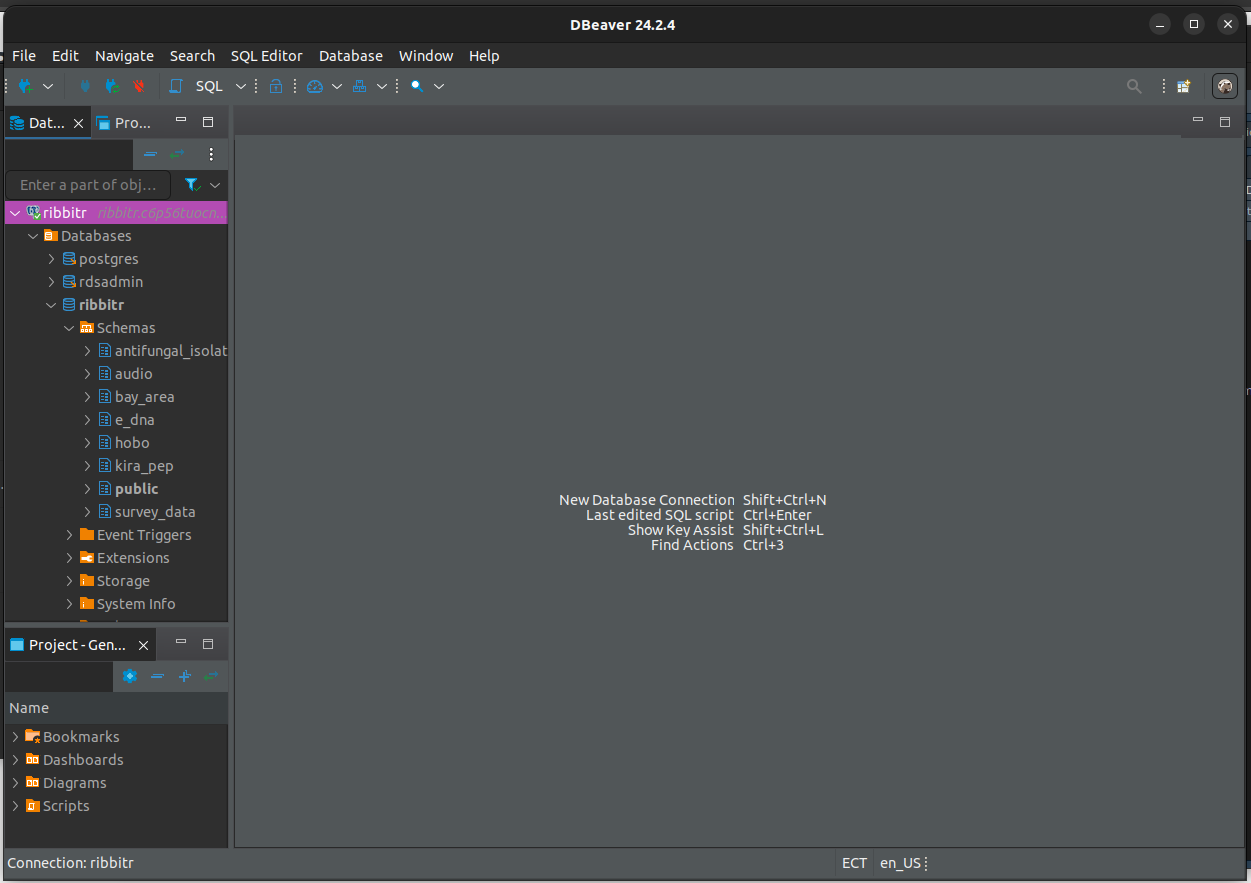
\includegraphics{images/DBeaver_data_discovery_01.png}

}

\caption{Navigate to \texttt{Databases} -\textgreater{} \texttt{ribbitr}
-\textgreater{} \texttt{Schemas}}

\end{figure}%

\subsubsection{Metadata: Data about
data}\label{metadata-data-about-data-2}

We keep track of information regarding what tables, and columns exist in
the database, and what information they are designed to describe, using
table and column metadata. To begin our process of data discovery, let's
learn what tables are present in the data by loading the table metadata.

\subsubsection{Table Metadata}\label{table-metadata-2}

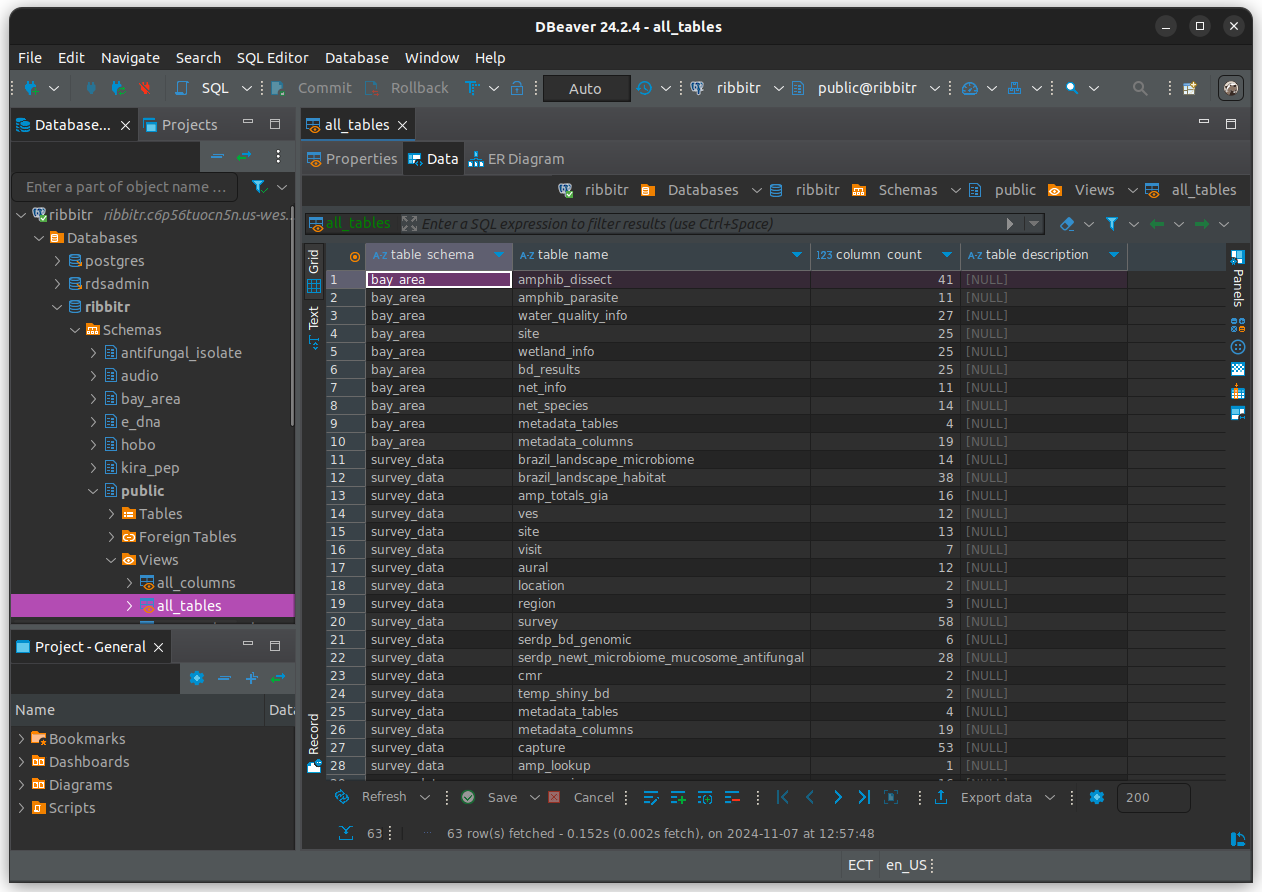
\includegraphics{images/DBeaver_data_discovery_02.png} See what you can
learn about the tables in the database form the table metadata.

\subsubsection{Column metadata}\label{column-metadata-2}

Suppose our interest is in the \texttt{survey\_data} schema. Let's take
a closer look at the tables here by collecting metadata on table columns
in this schema.

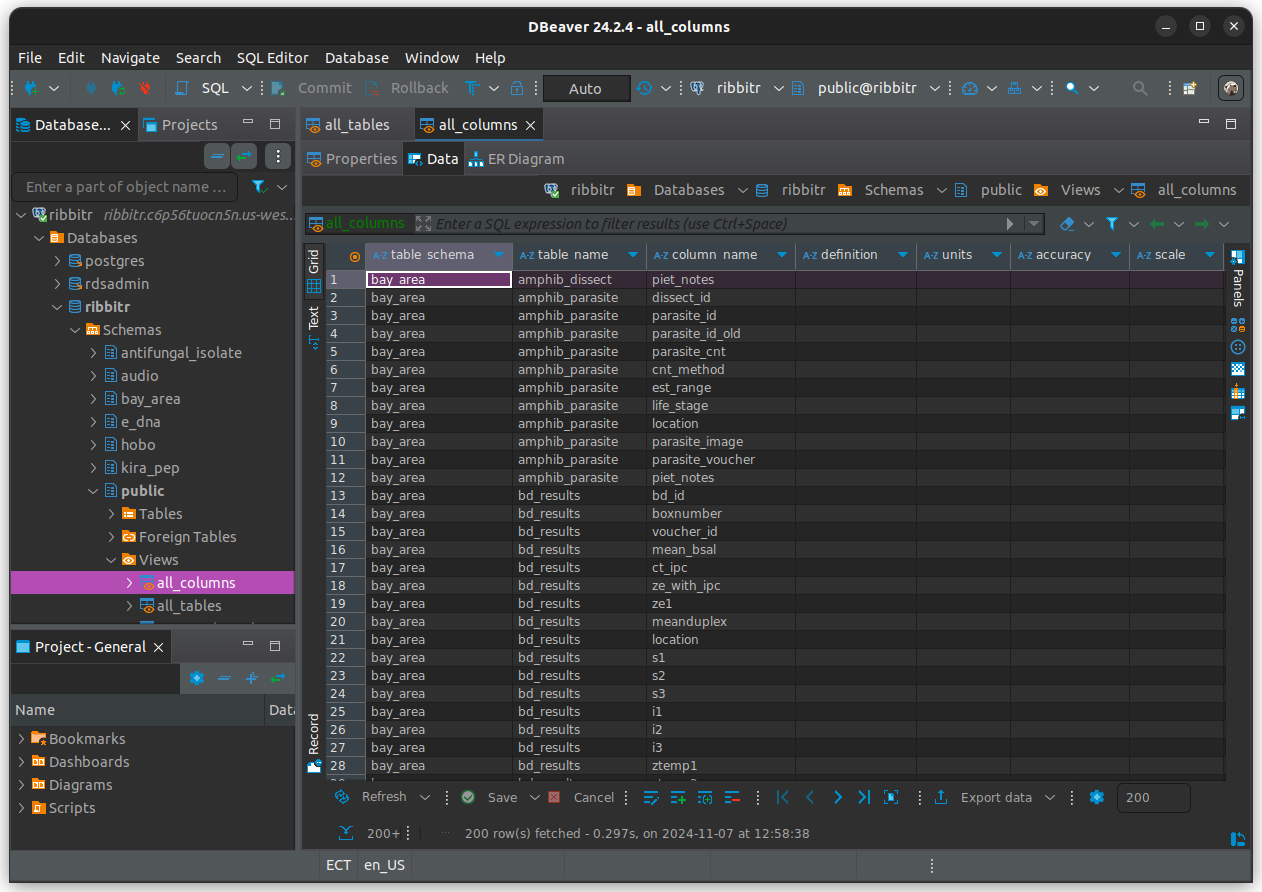
\includegraphics{images/DBeaver_data_discovery_03.png} Click on the
dropdown arrow next to \texttt{table\_schema}, click on
\texttt{Order\ by\ table\_schema\ ASC}. Repeat for the
\texttt{table\_name} and \texttt{column\_name} columns.

Scroll down until you see rows with \texttt{table\_schema} =
\texttt{survey\_data}. Explore a table of interest t see what you can
learn.

Curious about what a certain metadata column means? There's metadata for
that (metametadata?)! Scroll down to \texttt{table\_name} =
\texttt{metadata\_columns} to learn what the different columns in the
current table mean.

A few columns to point out:

\begin{itemize}
\tightlist
\item
  definition
\item
  units
\item
  data\_type
\item
  natural key
\end{itemize}

(more on keys later)

\subsection{Schema sructure}\label{schema-sructure}

\begin{figure}[H]

{\centering 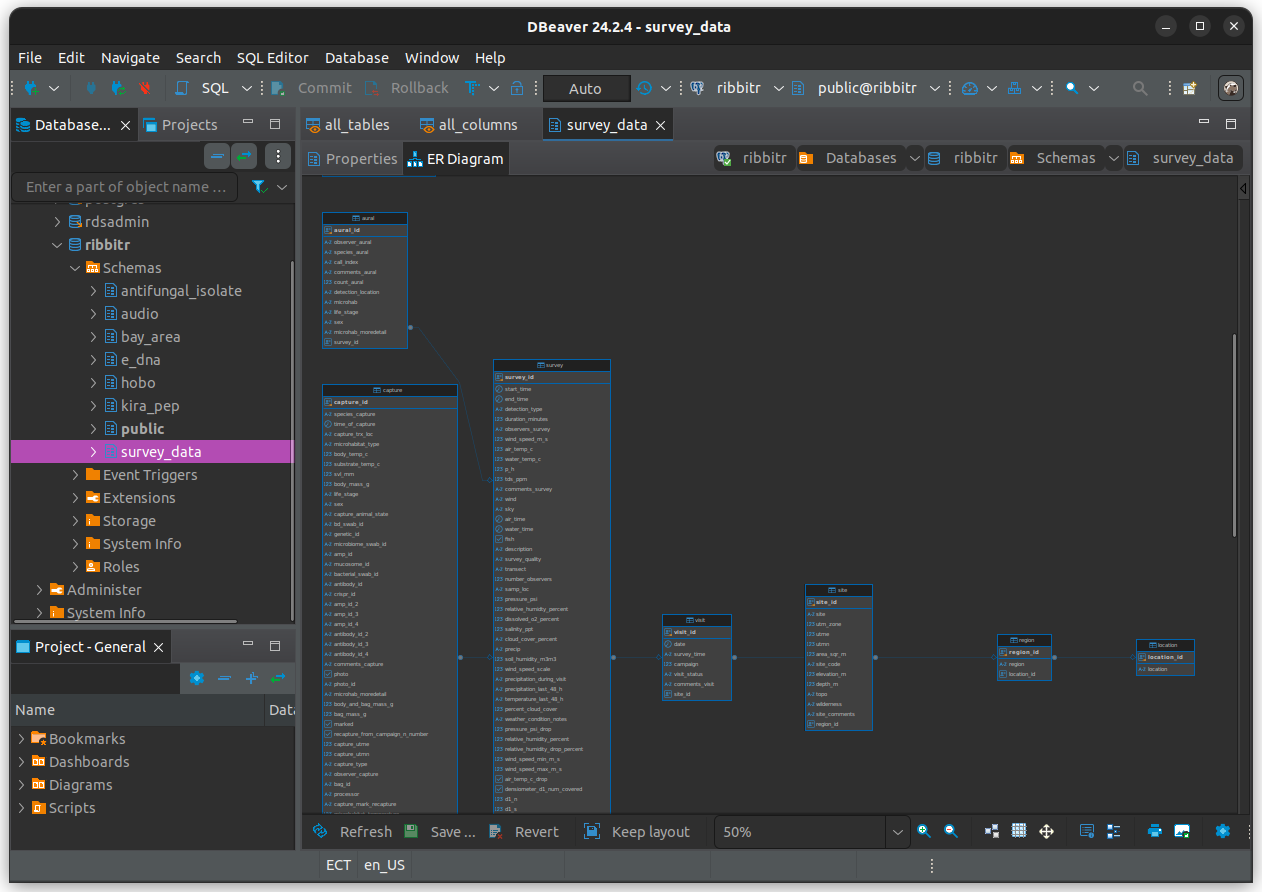
\includegraphics{images/DBeaver_data_discovery_04.png}

}

\caption{Navigate to \texttt{Databases} -\textgreater{} \texttt{ribbitr}
-\textgreater{} \texttt{Schemas} -\textgreater{} \texttt{survey\_data}.
Right-click and select \texttt{View\ Schema}. Select the
\texttt{ER\ Diagram} tab.}

\end{figure}%

This shows a diagram of the different tables within the
\texttt{surevy\_data} schema, as well as their columns and any
relationships between tables. This is a useful visual reference for
later, when we begin joining tables.

\subsection{Our first data table}\label{our-first-data-table-2}

To begin looking at data, let's navigate to the visual encounter surveys
(VES).

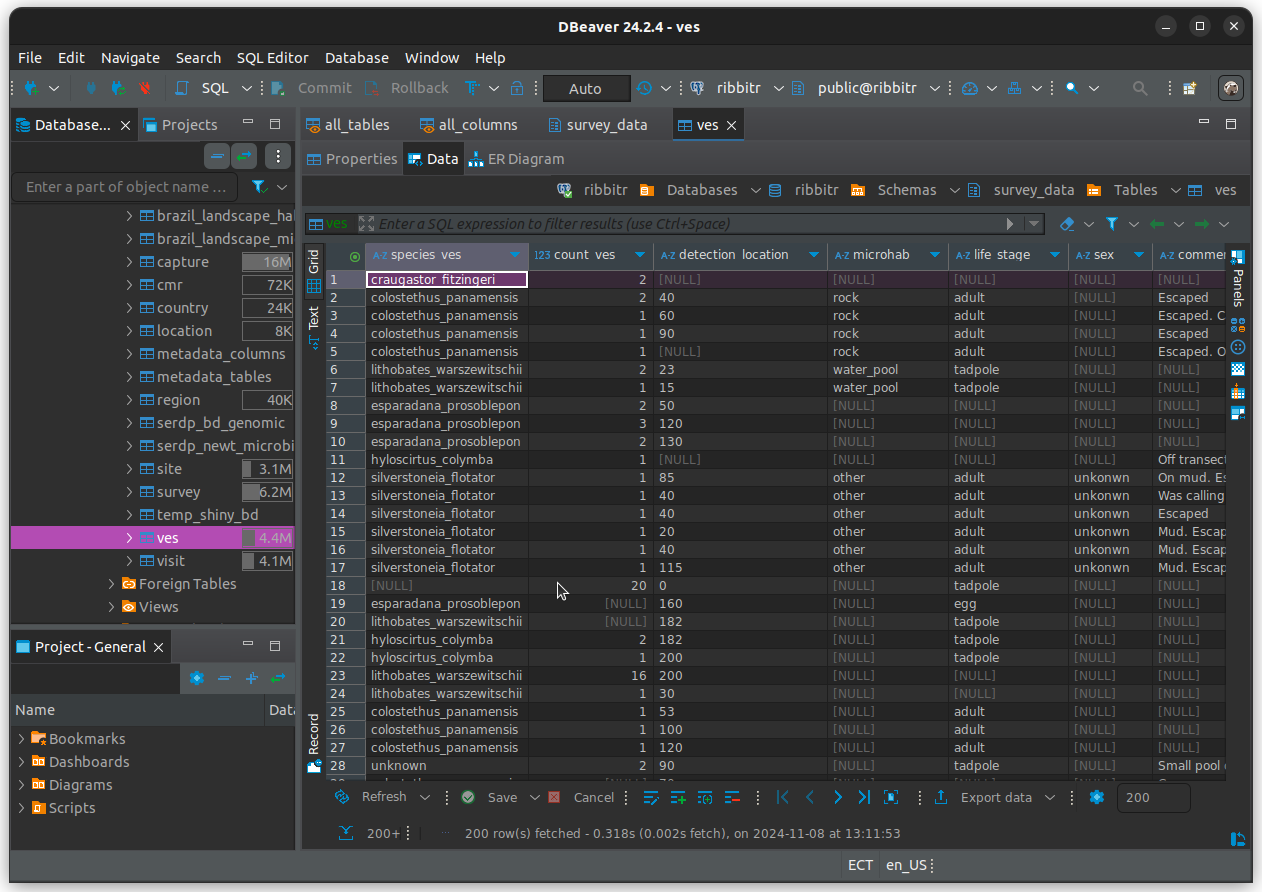
\includegraphics{images/DBeaver_data_discovery_05.png} This is your
first look at field data within the database! From here you can explore
organizing the data by columns, as well as exporting the table to a
.csv.

\href{01_connection_setup.html}{Previous Tutorial: Connection Setup}
\textbar{} \href{03_data_pulling.html}{Next Tutorial: Data Pulling}




\end{document}
